% 沿用 ex:interpretability-global-local；IG基准(0,0)，输入(1,1)，梯度(2,4)。
% 局部文字只是两个已定义二元特征的教学载体；贡献不是概率或现实因果量。
\begin{tikzpicture}[foundation picture,
 font=\figurefont\fontsize{8.5}{11}\selectfont,
 foundation heading/.append style={font=\figurefont\mdseries\fontsize{8.5}{11}\selectfont},
 foundation note/.append style={font=\FigureNoteFont\fontsize{8.5}{11}\selectfont}]
 \path[use as bounding box] (0,10) rectangle(119,71);
 \node at (55,66) {$f(x_1,x_2)=1+2x_1+4x_2$};
 \draw[FigureStroke,line width=.75pt,rounded corners=1.5mm] (1,20) rectangle(48,57);
 \node[foundation heading,anchor=west] at (5,51) {当前邮件$(1,1)$};
 \fill[FigureBlueFill,rounded corners=.6mm] (5,39) rectangle(43,46);
 \node[anchor=west] at (7,42.5) {支付要求：$x_1=1$};
 \fill[FigureRedFill,rounded corners=.6mm] (5,28) rectangle(43,35);
 \node[anchor=west] at (7,31.5) {可执行附件：$x_2=1$};
 \node[foundation note] at (24.5,14) {基准：两项均为0};
 \node[inner sep=0pt] at (88,36) {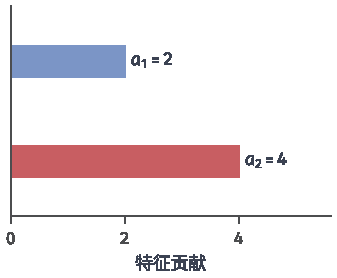
\includegraphics[width=57mm]{figures/02-foundations/03-trustworthiness/tikz/trust-feature-attribution/trust-feature-attribution.pdf}};
\draw[foundation flow,draw=FigureBlue] (49,42.5)--(56,42.5)--(56,49.16009)--(60.35217,49.16009);
\draw[foundation flow,draw=FigureRed] (49,31.5)--(57,31.5)--(57,32.28465)--(60.35217,32.28465);
\end{tikzpicture}